%! Author = gramic
%! Date = 24.03.24

% Preamble
\begin{flushleft}
    \subsection{Exkurs Architektur}
    In der Diplomarbeit werden diverse Konzepte und Begriffe behandelt.\\
    So wird das Partitioning, Sharding, Clusterkonzepte, Synchronisationen, Skalierungen und mehr Thema sein.\\
    Ziel von diesem Kapitel soll es sein, ein Verständnis für diese Konzepte zu schaffen.
%    %! Author = gramic
%! Date = 14.03.24

% Preamble
\subsubsection{ACID}
\label{ACID}
    \begin{description}
        \item \textbf{Atomicity}\hfill \\Besagt,
        \item \textbf{Consistency}\hfill \\B
        \item \textbf{Isolation}\hfill \\Beschreibt,
        \item \textbf{Durability}\hfill \\Sagt aus,
    \end{description}

    %! Author = gramic
%! Date = 19.03.24

% Preamble
\begin{flushleft}
    \subsubsection{Sharding}
    \paragraph{Vertikales / Horizontales Sharding}
    Tabellen können Horizontal oder Vertikal partitioniert werden.
    \begin{figure}[H]
        \centering
        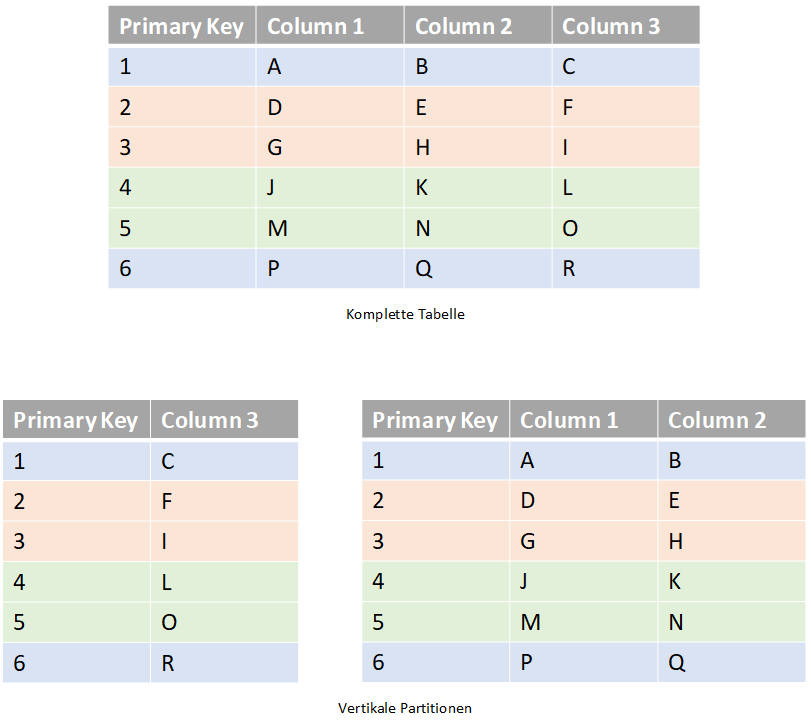
\includegraphics[width=0.8\linewidth]{source/implementation/evaluation/excursus_architecture/sharding_vertical_partitioning}
        \caption{Sharding - Vertikale Partitionierung}
        \label{fig:sharding_vertical_partitioning}
    \end{figure}
    \begin{figure}[H]
        \centering
        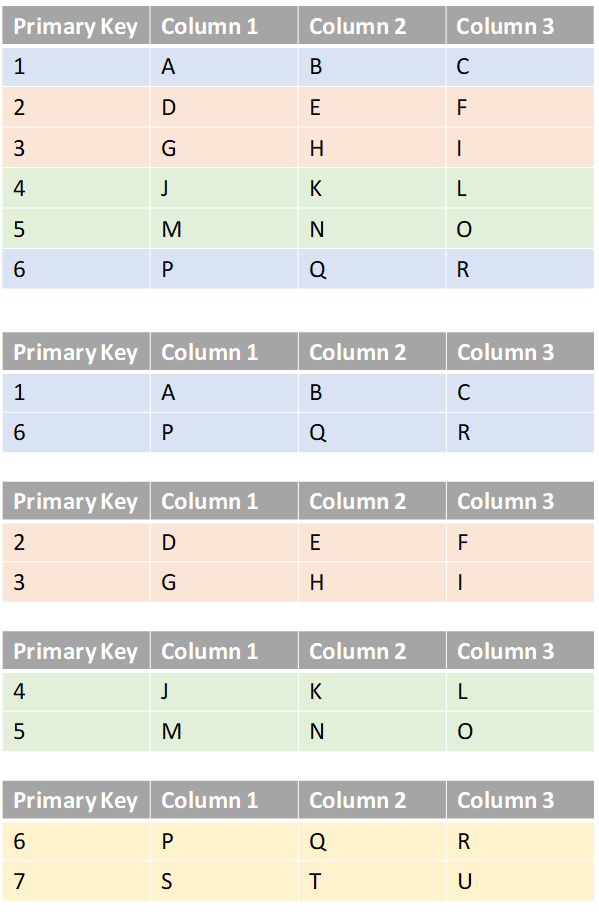
\includegraphics[width=0.8\linewidth]{source/implementation/evaluation/excursus_architecture/sharding_horizontal_partitioning}
        \caption{Sharding - Horizontales Partitionierung}
        \label{fig:sharding_horizontal_partitioning}
    \end{figure}
    Horizontales Partitionieren wird meistens für das Sharding von Tabellen benutzt.
    Die Partitionen entsprechen dann den Shards.
\begin{flushleft}
\end{flushleft}
    \paragraph{Key Based Sharding}
    Hierbei wird das sharding anhand eines oder mehreren Keys ausgeführt.
\begin{flushleft}
\end{flushleft}
    \paragraph{Range Based Sharding}
    Das Sharding wird dabei anhand von Ranges ausgeführt.
    Zum Beispiel anhand von Preis-Ranges.
\begin{flushleft}
\end{flushleft}
    \paragraph{Directory Based Sharding}
    Hierfür wird eine lookup-Tabelle geführt, welche die Schlüssel für das Sharding bereitstellen.
    Anhand dieser werden dann die entsprechenden Zieltabellen aufgeteilt.
\begin{flushleft}
\end{flushleft}
    \paragraph{Hash Based Sharding}
    Das Hash Based Sharding ist eine Form des Range Based Shardings, bei dem Hashwerte der Datensätze benutzt werden.
    Je nach Bereich wird der Datensatz dann einem Shard zugewiesen.
\end{flushleft}
    %! Author = itgramic
%! Date = 05.12.23

% Preamble
\subsubsection{Monolithische vs. verteilte SQL Systeme}
Klassische SQL-Datenbanken sind Monolithische Systeme, selbst wenn sie mittels Replikation eine Primary/Standby-Architektur aufweisen.
Man kann mittels eines SQL Proxys ein gewisses Mass an Load Balancing betreiben, hat aber immer noch das Problem das es einen Primary Node gibt auf dem beschrieben wird.

Verteilte Systeme wiederum

\begin{figure}[H]
    \centering
    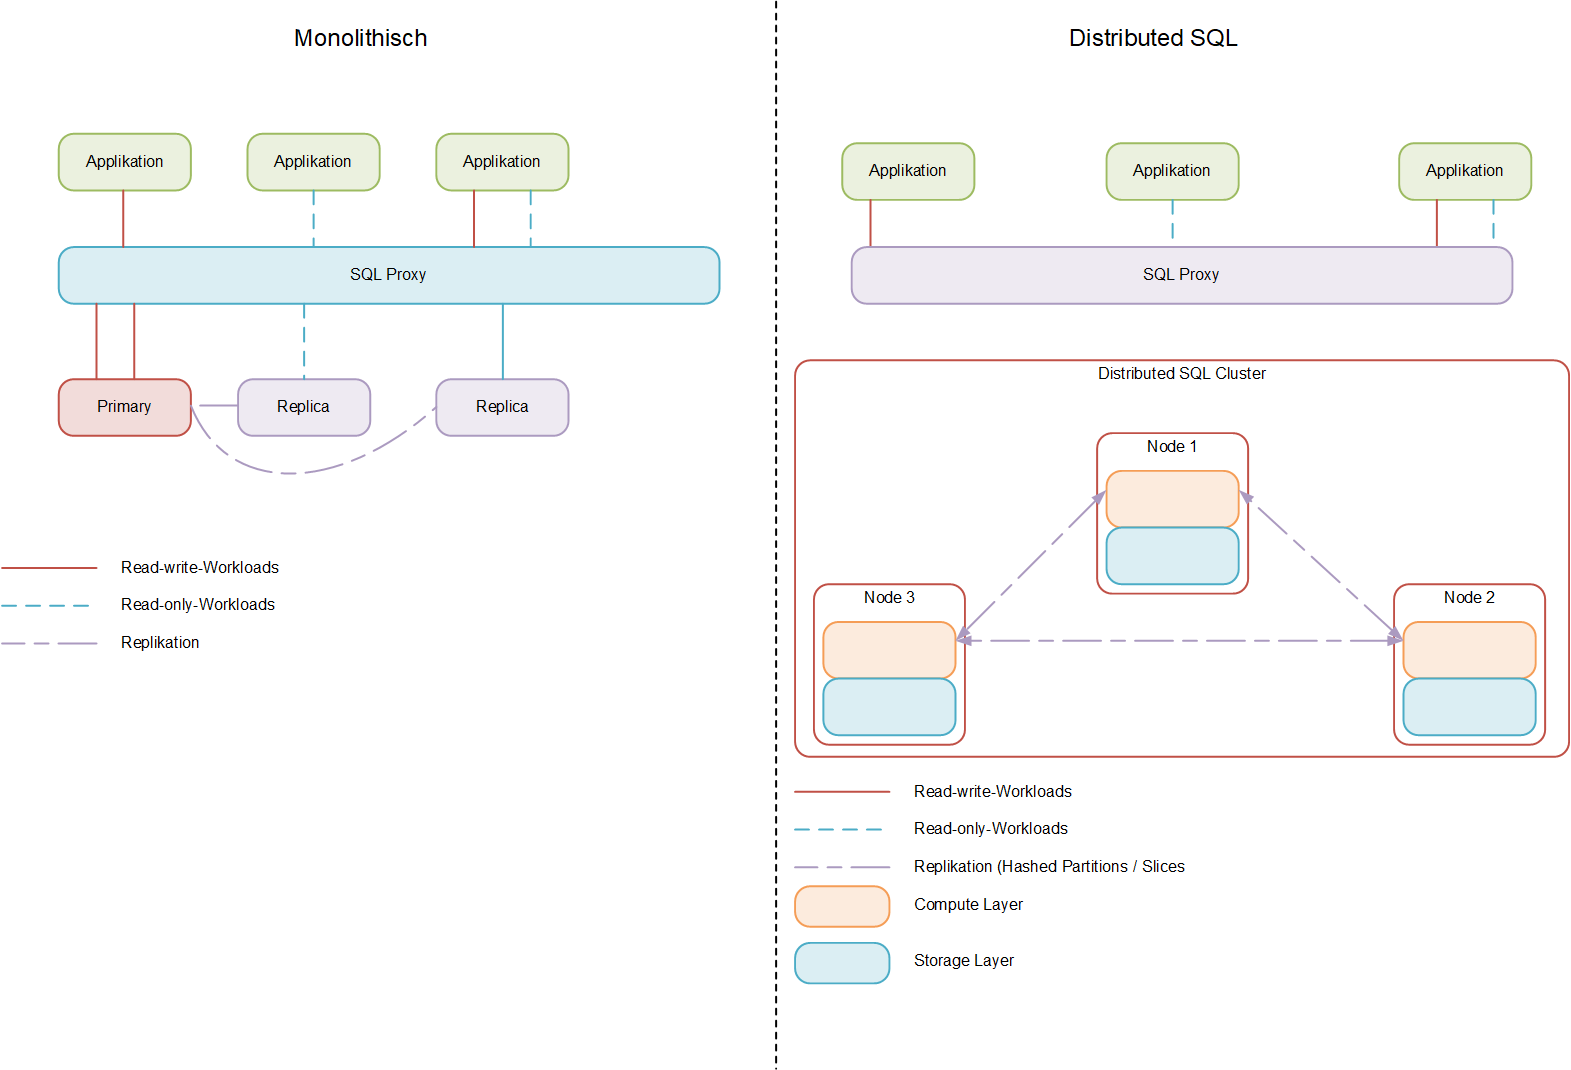
\includegraphics[width=1\linewidth]{source/implementation/evaluation/excursus_architecture/monolith_distributed}
    \caption{Monolithische vs. verteilte SQL Systeme}
    \label{fig:Monolith_vs_Distributed_SQL}
\end{figure}

    %! Author = itgramic
%! Date = 05.12.23

% Preamble
\subsubsection{High Availability und Replikation}
\begin{flushleft}
    Wenn eine Datenbank HA (High Availability), also Hochverfügbar, sein soll, braucht es eine Primäre und mindestens eine Sekundäre- oder \Gls{Failover}-Datenbank.
    Um Datenverlust zu vermeiden, müssen die Daten permanent von der Primären auf die sekundäre Datenbank repliziert werden, dies nennt man Replikation\cite{D9RDXENY}.
    Dabei wird zwischen den folgenden beiden Replikationen unterschieden:
\end{flushleft}
\begin{flushleft}
    \textbf{Synchrone Replikation}\\
    Wenn bei einer Synchronen Replikation eine Transaktion abgesetzt wird, wird der Commit auf der primären Seite erst gesetzt, wenn die Änderung auf der sekundären Seite oder den sekundären Seiten ebenfalls eingetragen und Committed ist.
    Bis zu diesem Moment ist die Transaktion nicht als Committed.
    
    Dies wird dann zum Problem, wenn keine Verbindung mehr zu mindesten einer sekundären Seite vorhanden ist.
    Zudem wird die Synchrone Replikation bei hohen Latenzen zum Bottleneck der Datenbank.
\end{flushleft}
\begin{flushleft}
    \textbf{Asynchrone Replikation}\\
    Bei der Asynchronen Replikation wird eine Transaktion erst auf der eigenen primären Seite Committed und erst dann an die sekundären Nodes gesendet.
    Besonders bei hohen Latenzen bleibt die Datenbank immer perfomant, allerdings kann es je nach Latenz und genereller Auslastung zu Datenverlusten kommen, wenn es zum \Gls{Failover} kommt.
\end{flushleft}
    %! Author = itgramic
%! Date = 05.12.23

% Preamble
\subsubsection{Quorum}
\label{subsubsec:quorum}
\begin{flushleft}
    Ein Quorum-System soll die Integrität und Konsistenz in einem Datenbank-Cluster sicherstellen.
    Dabei gilt zu beachten, das nicht eine beliebige Anzahl an Nodes hinzugefügt werden können.
    Auch hat das Hinzufügen von Nodes immer eine Einbusse an Performance zur Folge, besonders dann, wenn eine synchrone Replikation gewählt wird und auf jedes Commitment von den Replica-Nodes gewartet werden muss.

    \begin{description}
        \item \textbf{Quorum}\hfill \\Die Mehrheit der Server, die einen funktionierenden Betrieb gewährleisten können, ohne eine \Gls{Split-brain}-Situation zu erzeugen.
        Die Formel ist gemeinhin \(n/2 + 1\)
        \item \textbf{Throughput}\hfill \\Beschreibt, wie sich die Anzahl Nodes auf die Schreibgeschwindigkeit der Commitments auf die restlichen Nodes auswirkt.\\Die Verdopplung der Server halbiert i. d. R. den Throughput.
        \item \textbf{Fehlertoleranz}\hfill \\Beschreibt, wie viele Nodes ausfallen können, damit der Cluster noch arbeitsfähig ist.\\Wobei eine Erhöhung der Nodes von 3 auf 4 die Fehlertoleranz nicht erhöht, da nun eine \Gls{Split-brain}-Situation entstehen kann.
    \end{description}
    %\begin{landscape}
    %\begin{table}[]
    %\resizebox{\columnwidth}{!}{%
    %\begin{tabular}{@{}llll@{}}
    %\toprule
    %\textbf{Anzahl Nodes} & \textbf{Quorum} & \textbf{Fehlertoleranz} & \textbf{Representative Throughput} \\ \midrule
    %1                     & 1               & 0                                               & 100                                \\
    %2                     & 2               & 0                                               & 85                                 \\
    %3                     & 2               & 1                                               & 82                                 \\
    %4                     & 3               & 1                                               & 57                                 \\
    %5                     & 3               & 2                                               & 48                                 \\
    %6                     & 4               & 2                                               & 41                                 \\
    %7                     & 4               & 3                                               & 36                                 \\ \bottomrule
    %\end{tabular}%
    %}
    %\caption{Quorum Beispiele}
    %\label{tab:quorum-beispiele}
    %\end{table}
    %\end{landscape}
    %\subsubsection{Split-brain}
    %\label{chap:Split-brain}
    Hier ein Beispiel wie sie in den Artikeln \cite{UMIGLCCI, YDS7DTYM, V4XLXN7W} beschrieben werden.
    Es zeigt auf, ab wie vielen Nodes die Fehlertoleranz erhöht wird und wie sich der repräsentative Throughput verhält.
%\end{flushleft}
%\begin{flushleft}
    \begin{table}[H]
    \resizebox{\columnwidth}{!}{%
    \begin{tabular}{@{}llll@{}}
    \toprule
    \textbf{Anzahl Nodes} & \textbf{Quorum} & \textbf{Fehlertoleranz} & \textbf{Representative Throughput} \\ \midrule
    1                     & 1               & 0                       & 100                                \\
    2                     & 2               & 0                       & 85                                 \\
    3                     & 2               & 1                       & 82                                 \\
    4                     & 3               & 1                       & 57                                 \\
    5                     & 3               & 2                       & 48                                 \\
    6                     & 4               & 2                       & 41                                 \\
    7                     & 4               & 3                       & 36                                 \\ \bottomrule
    \end{tabular}%
    }
    \caption{Quorum Beispiele}
    \label{tab:quorum-beispiele}
    \end{table}
\end{flushleft}
    %! Author = itgramic
%! Date = 05.12.23

% Preamble
\subsubsection{CAP Theorem}
Das CAP Theorem besagt, das nur zwei der drei folgenden drei Merkmale von verteilten Systeme gewährleistet werden können\cite{EE6EQHU2}.
\begin{flushleft}
\textbf{Konsistenz - Consistency}\\
    Die Datenbank ist Konsistent, alle Clients seher gleichzeitig die gleichen Daten unabhängig auf welchem Node Zugegriffen wird.
    Hierzu muss eine Replikation der Daten an alle Nodes stattfinden und der Commit zurückgegeben werden, also eine Synchrone Replikation stattfinden.
\end{flushleft}
\begin{flushleft}
\textbf{Verfügbarkeit - Availability}\\
    Jeder Client, der eine Anfrage sendet, muss auch eine Antwort erhalten.
    Unabhängig davon wie viele Nodes im Cluster noch aktiv ist.
\end{flushleft}
\begin{flushleft}
\textbf{Ausfalltoleranz / Partitionstoleranz - Partition tolerance}\\
    Der Cluster muss auch dann noch funktionsfähig bleiben, wenn es eine beliebige Anzahl von Verbindungsunterbrüchen oder anderen Netzwerkproblemen zwischen den Nodes gibt.

\end{flushleft}
\begin{flushleft}
    \begin{figure}[H]
        \centering
        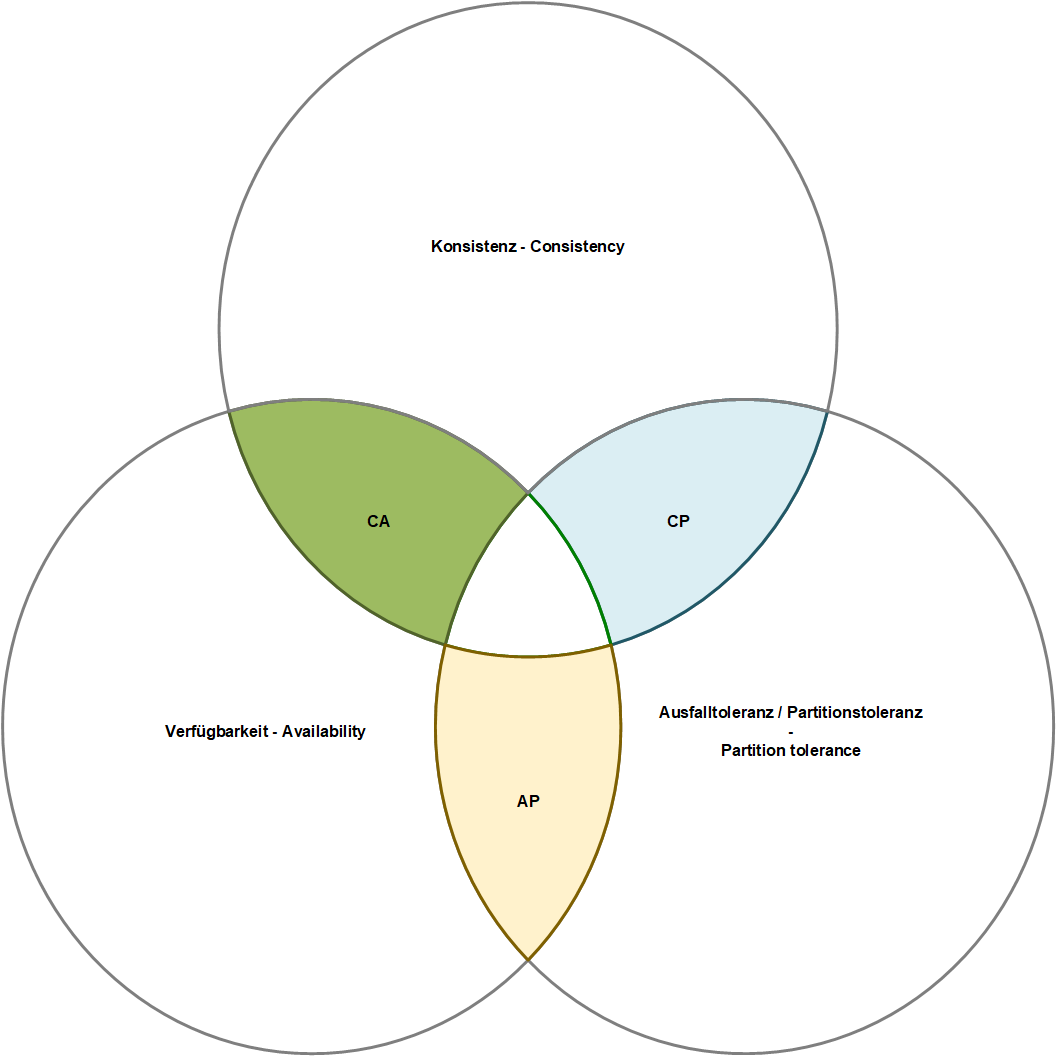
\includegraphics[width=0.5\linewidth]{source/implementation/evaluation/excursus_architecture/cap_theorem}
        \caption{CAP-Theorem}
        \label{fig:cap_theorem}
    \end{figure}

    \Gls{PostgreSQL}, \Gls{Oracle Database} oder \Gls{IBM DB2} präferieren CA, also Konsistenz und Verfügbarkeit.
\end{flushleft}
    %! Author = itgramic
%! Date = 05.12.23

% Preamble
\subsubsection{Skalierung}
Datenbanken müssen skalierbar sein.
Dabei wird unterschieden zwischen einer vertikalen Skalierung (scale-up) und horizontaler Skalierung (scale-out).
Bei der vertikalen Skalierung werden den DB-Servern mehr CPU-Cores und Memory sowie zum Teil Storage hinzugefügt, wobei der Storage in jedem Fall wachsen wird.
Beim horizontalen Skalieren werden weitere DB-Nodes in den Cluster eingehängt\cite{IZSGZLVT}:
\begin{figure}[H]
    \centering
    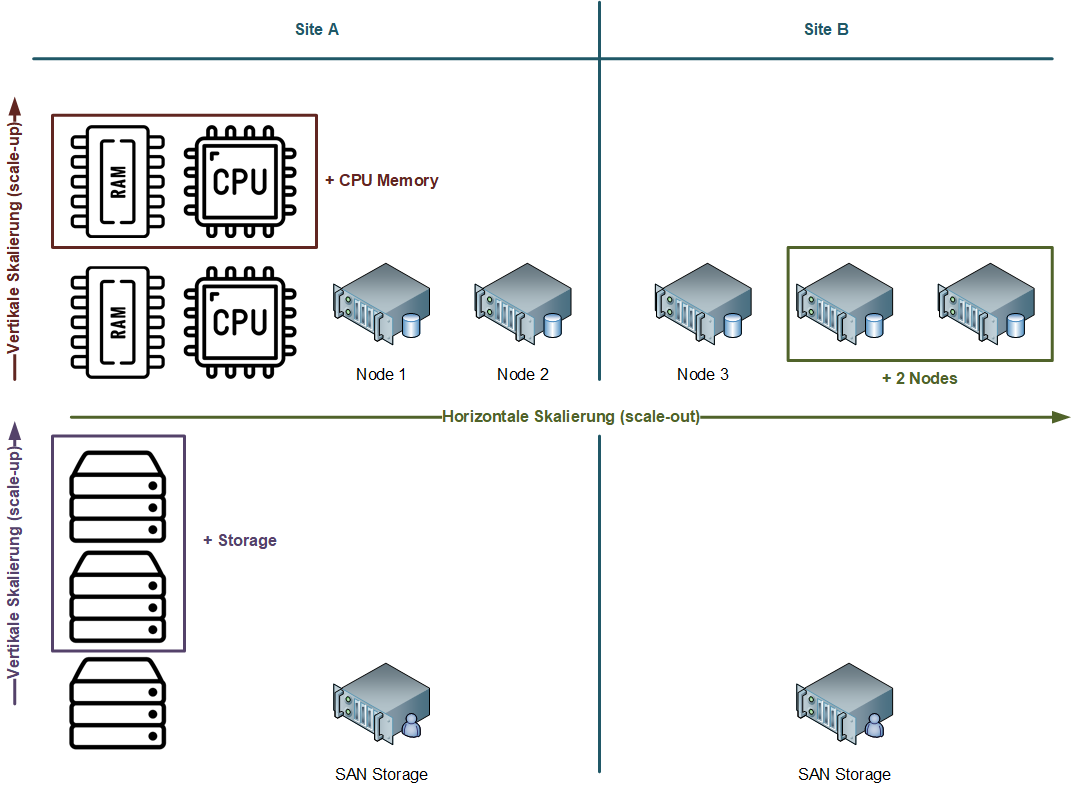
\includegraphics[width=1\linewidth]{source/implementation/evaluation/excursus_architecture/Skalierung}
    \caption{Datenbankskalierung}
    \label{fig:Datenbankskalierung}
\end{figure}

Bei monolithischen Datenbanken, werden irgendwann die grenzen der horizontalen Skalierung erreicht und man muss wieder vertikal Skalieren, um dem Primary Node genügend Rechnerleistung vorzuhalten.
\end{flushleft}